\chapter{Disturbance Model Identification}
\label{chap-identification}

\section{Identifying disturbance models}

t.b.d. —depends if we identify useful methods.

Outline notes:
\begin{outline}
	\1 Test methods of identifying the disturbance model parameters from simulated measurements.
	\2 Using data from linear system from section 2.1.
	\2 Using data from grinding model simulations from section 2.3.
	\1 Results of identifying the random shock distribution with noise using Expectation-Maximization (EM) algorithm to fit Gaussian Mixture models.
	\1 Problem of inference of the RODD - simply inverting model magnifies noise.
	\1 Eriksson and Isaksson's approach to system detection. Using an observer to identify system from a set of known systems.
	\1 Demos of other methods:
	  \2 Total variation de-noising (for step disturbance signals)
	  \2 Variational inference (how is this different from EM?)
	\1 Sequential inference techniques? E.g. Sequential Monte Carlo. Don't know enough about this. Mention in conclusion and recommendations for future work.
\end{outline}

\section{Characterizing ore disturbances from operating data}

t.b.d. —depends if the data is good enough for the purpose.

Outline notes:
\begin{itemize}
	\item Description of plant and data acquisition process.
	\item Preparation and pre-processing of data—outliers, missing values, standardization parameters.
	\item Ideally: Demonstrate disturbance characterisation (model structure), identification (parameters) with one or more method and discuss results. 
\end{itemize}

For the purposes of this work, efforts were made to acquire data on ore properties and operating conditions from other operations. A set of hourly data on ore properties was provided by one mining operation. For commercial reasons, details of the source of this data cannot be disclosed and the data has been normalized and de-trended to remove important features. \textbf{TODO: GET PERMISSION TO SHARE—MAY NOT BE POSSIBLE}. A sample of this adjusted data is shown in Figure \ref{fig:dist_sample}. The two variables are indicators of the ore properties at the feed to the concentrator plant---particle size and hardness. The particle size indicator is based on a real-time measurement---a specialised camera image-based system that provides a dimensionless particle size indication (higher values indicates larger particles). The hardness variable is also a dimensionless indicator produced by a customized operational forecasting model which incorporates data from a variety of sources, including geological data and data from recent drilling activities. The source data is time-delayed according to a model of the flows of material through the mining and ore feed system, therefore this variable is a prediction based on past data inputs and may not reflect current conditions or the actual variability in the feed stream.

\begin{figure}[htp]
	\centering
	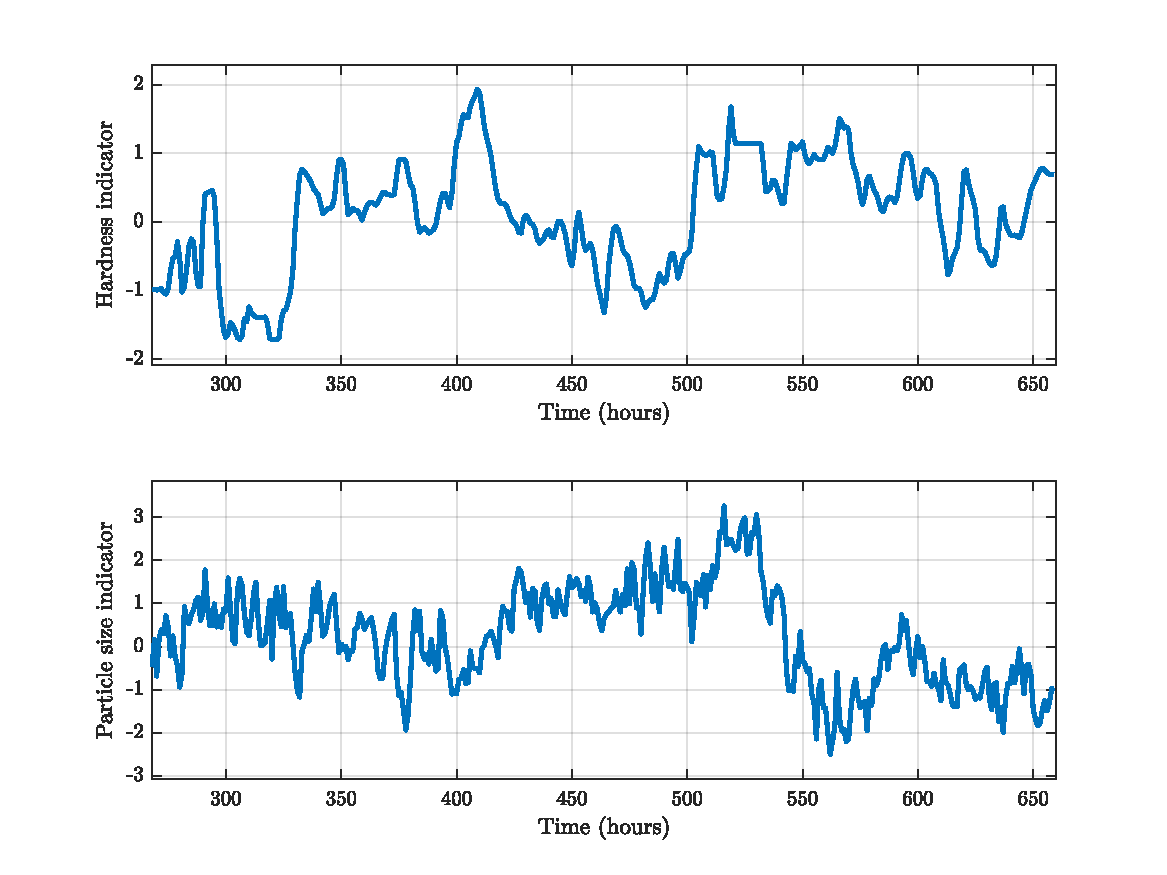
\includegraphics[width=15cm]{images/ind-data-snapshot-tsplot.pdf}
	\caption{Sample of ore data from a mine}
	\label{fig:dist_sample}
\end{figure}

There is a limit to what can be deduced from one data sample. Nevertheless, it provides a rare insight into the nature of ore variability. In the case of the hardness indicator, abrupt changes are visible, interspersed by periods of lower variance between one trend and the next. For example, for roughly the first 50 hours the particle size exhibits an increasing trend, whereas from roughly 50 hour point to 170 hours it exhibits a declining trend. Around the 300-hour mark, a rapid decline occurs lasting about 20 hours. In addition to these obvious trends, there is considerable variability at higher frequencies, which is harder to characterize by eye. Since the data are hourly samples, they provide no indication of variations that may occur at higher frequencies. Higher frequency variations may be more important for process control design.

